\documentclass[%
    a4paper,              % DIN A4
    style=screen,          % print: enables twoside, print colors, and BCOR=15mm
    bibliography=totoc,   % bibliography gets unnumbered entry
    nexus,                % corporate design font
    lnum,                 % use "Versalziffern" instead of "Mediaevalziffern"
    extramargin,          % override corporate design margin to give more space for one-column text
]{tubsbook}

%\usepackage[T1]{fontenc}
\usepackage[utf8]{inputenc}

\usepackage{float}
%\usepackage{pgfplots}
\usepackage{microtype}
\usepackage{xcolor}
    \definecolor{medium-blue}{rgb}{0,0,0.5}
\usepackage{algorithm}
\usepackage{algpseudocode}
    \renewcommand{\algorithmicrequire}{\textbf{Input:}}
    \renewcommand{\algorithmicensure}{\textbf{Output:}}
\usepackage{hyperref}
\usepackage{amsmath}
\usepackage{amsthm}
\usepackage{mathtools}
    \mathtoolsset{centercolon}
\usepackage[nameinlink]{cleveref}
    \newtheorem{theorem}{Theorem}
    \newtheorem{corollary}{Corollary}
    \theoremstyle{definition}
    \newtheorem{definition}{Definition}
    \newtheorem{lemma}{Lemma}
    \newtheorem{problem}{Problem}
    \newtheorem{conjecture}{Conjecture}
\usepackage{amsfonts}
%\usepackage{todonotes}
\usepackage{subcaption}
\usepackage{tikz}
    \usetikzlibrary{calc}
    \usetikzlibrary{arrows}
    \usetikzlibrary{decorations.pathreplacing}
    %\usetikzlibrary{external}
    %\tikzexternalize[prefix=tikz/]
    \newcommand\fig[3][3]{%
        \begin{figure}%
            %\tikzsetnextfilename{#1}%
            \begin{tikzpicture}[scale=#1]%
                \input{tikz/#2.tex}%
            \end{tikzpicture}%
            \caption{#3}%
            \label{fig:#2}%
        \end{figure}%
    }
    \newcommand\subfig[2][3]{%
        %\tikzsetnextfilename{#1}%
        \begin{tikzpicture}[scale=#1]%
            \input{tikz/#2.tex}%
        \end{tikzpicture}%
    }
\usepackage{graphicx}
    \graphicspath{{images/}}
\usepackage{longtable}
    \renewcommand{\arraystretch}{2}
\usepackage{chngcntr}
    \counterwithout{equation}{chapter}
\usepackage{nicefrac}
\usepackage{csquotes}
\usepackage{scrhack}
\usepackage{array}
\usepackage{xifthen}
\usepackage[backend=biber,style=numeric-comp,maxbibnames=99,url=false]{biblatex}
    \addbibresource{references.bib}

    %% Link complete "Author (Year)", not just "(Year)"
    %\DeclareFieldFormat{citehyperref}{%
    %  \DeclareFieldAlias{bibhyperref}{noformat}% Avoid nested links
    %  \bibhyperref{#1}}

    %\DeclareFieldFormat{textcitehyperref}{%
    %  \DeclareFieldAlias{bibhyperref}{noformat}% Avoid nested links
    %  \bibhyperref{%
    %    #1%
    %    \ifbool{cbx:parens}
    %      {\bibcloseparen\global\boolfalse{cbx:parens}}
    %      {}}}

    %\savebibmacro{cite}
    %\savebibmacro{textcite}

    %\renewbibmacro*{cite}{%
    %  \printtext[citehyperref]{%
    %    \restorebibmacro{cite}%
    %    \usebibmacro{cite}}}

    %\renewbibmacro*{textcite}{%
    %  \ifboolexpr{
    %    ( not test {\iffieldundef{prenote}} and
    %      test {\ifnumequal{\value{citecount}}{1}} )
    %    or
    %    ( not test {\iffieldundef{postnote}} and
    %      test {\ifnumequal{\value{citecount}}{\value{citetotal}}} )
    %  }
    %    {\DeclareFieldAlias{textcitehyperref}{noformat}}
    %    {}%
    %  \printtext[textcitehyperref]{%
    %    \restorebibmacro{textcite}%
    %    \usebibmacro{textcite}}}

\widowpenalty10000
\clubpenalty10000

\newcommand{\C}{\mathbb{C}}
\newcommand{\R}{\mathbb{R}}
\newcommand{\myS}{\mathbb{S}}
\newcommand{\s}{\sqrt{2}}
\newcommand{\wlofg}{without loss of generality}
\DeclareMathOperator{\mysum}{sum}
\DeclareMathOperator*{\argmin}{arg\,min}

\newcommand{\entry}[7]{
\begin{tikzpicture}[scale=#1,baseline={([yshift={-\ht\strutbox}]current bounding box.north)}]\input{tikz/#2.tex}\end{tikzpicture}
& \textbf{#3} (#4) \vfill\vspace{10pt}
\ifthenelse{\isempty{#5}}{}{\textit{Condition:} #5 \vfill\vspace{5pt}}
\textit{Density:} #6 \vfill\vspace{5pt}
\textit{Approximation factor:} #7\\
}

\makeatletter
    % center the contents of floatstuff automatically
    \g@addto@macro\@floatboxreset\centering

    % set default placement for floatstuff
    \def\fps@figure{H}
    \def\fps@table{H}
    \def\fps@algorithm{H}
\makeatother

%%%%%%%%%%%% TikZ %%%%%%%%%%%%%%%

\newcommand{\B}{1.36207}

\tikzset{tight/.style={inner sep=1pt}}
\tikzset{bracket/.style={inner sep=10pt,draw=gray,decorate,decoration={brace,amplitude=5pt}}}
\tikzset{helper/.style={dashed}}
\tikzset{filled/.style={fill=black!40!white}}
\tikzset{filled2/.style={fill=black!15!white}}
\tikzset{cover/.style={fill=black!30!white,fill opacity=0.5}}

%\newcommand\hatshape[3][]{
%    \pgfmathsetmacro{\r}{sqrt((#2)/pi)}
%    \pgfmathsetmacro{\s}{sqrt((#3)/pi)}
%
%    \coordinate (top) at (0,{(\r/(sqrt(2)-1)});
%    \coordinate (right) at ({(\r/(sqrt(2)-1)},0);
%    \coordinate (left) at ({(-\r/(sqrt(2)-1)},0);
%
%    \coordinate (leftcenter) at ($({-(\r-\s)/(sqrt(2)-1)},0)+(0,\s)$);
%    \coordinate (leftbottom) at ($(leftcenter)+(-90:\s)$);
%    \coordinate (lefttop) at ($(leftcenter)+(-225:\s)$);
%
%    \coordinate (rightcenter) at ($({(\r-\s)/(sqrt(2)-1)},0)+(0,\s)$);
%    \coordinate (rightbottom) at ($(rightcenter)+(-90:\s)$);
%    \coordinate (righttop) at ($(rightcenter)+(45:\s)$);
%
%    \coordinate (midcenter) at (0,\r);
%
%    \draw[#1] (rightbottom) arc (-90:45:\s) -- (top) -- (lefttop) arc (-225:-90:\s) -- cycle;
%}

\newcommand\hatshape[5][]{
    \pgfmathsetmacro{\r}{sqrt((#2)/pi)}
    \pgfmathsetmacro{\s}{sqrt((#3)/pi)}
    \pgfmathsetmacro{\a}{(#4)}
    \pgfmathsetmacro{\b}{(#5)}

    \coordinate (top) at ({cos((90+(\a-\b)/2))*(\r/cos((\a+\b)/2))},{sin((90+(\a-\b)/2))*(\r/cos((\a+\b)/2)});
    \coordinate (left) at ({-\r/tan(\a/2)},-\r);
    \coordinate (right) at ({\r/tan(\b/2)},-\r);

    \coordinate (leftcenter) at ($(left)+({\s/tan(\a/2)},\s)$);
    \coordinate (leftbottom) at ($(leftcenter)+(-90:\s)$);
    \coordinate (lefttop) at ($(leftcenter)+({-270+\a}:\s)$);

    \coordinate (rightcenter) at ($(right)+({-\s/tan(\b/2)},\s)$);
    \coordinate (rightbottom) at ($(rightcenter)+(-90:\s)$);
    \coordinate (righttop) at ($(rightcenter)+({90-\b}:\s)$);

    \coordinate (topcenter) at ($(top)-({cos((90+(\a-\b)/2))*(\s/cos((\a+\b)/2))},{sin((90+(\a-\b)/2))*(\s/cos((\a+\b)/2)})$);
    \coordinate (topleft) at ($(topcenter)+({-270+\a}:\s)$);
    \coordinate (topright) at ($(topcenter)+({90-\b}:\s)$);

    \coordinate (midcenter) at (0,0);

    %\draw[#1] (right) -- (top) -- (left) -- cycle;
    \draw[#1] (rightbottom) arc (-90:{90-\b}:\s) -- (topright) arc ({90-\b}:{90+\a}:\s) -- (lefttop) arc ({-270+\a}:-90:\s) -- cycle;
}
\newcommand\gemshape[3][]{
    \pgfmathsetmacro{\r}{sqrt((#2)/pi)}
    \pgfmathsetmacro{\s}{sqrt((#3)/pi)}
    \pgfmathsetmacro{\l}{0.85955*sqrt(#3)}
    \pgfmathsetmacro{\ll}{0.7654*\l}
    \pgfmathsetmacro{\a}{45}
    \pgfmathsetmacro{\b}{45}

    \coordinate (top) at ({cos((90+(\a-\b)/2))*(\r/cos((\a+\b)/2))},{sin((90+(\a-\b)/2))*(\r/cos((\a+\b)/2)});
    \coordinate (left) at ({-\r/tan(\a/2)},-\r);
    \coordinate (right) at ({\r/tan(\b/2)},-\r);

    \coordinate (leftcenter) at ($(left)+({\s/tan(\a/2)},\s)$);
    \coordinate (lefttop) at ($(left)+(45:\l)$);
    \coordinate (leftmid) at ($(left)+(22.5:\ll)$);
    \coordinate (leftbottom) at ($(left)+(0:\l)$);

    \coordinate (rightcenter) at ($(right)+({-\s/tan(\b/2)},\s)$);
    \coordinate (righttop) at ($(right)+(135:\l)$);
    \coordinate (rightmid) at ($(right)+(157.5:\ll)$);
    \coordinate (rightbottom) at ($(right)+(180:\l)$);

    \coordinate (midcenter) at (0,0);

    \draw[#1] (top) -- (righttop) -- (rightmid) -- (rightbottom) -- (leftbottom) -- (leftmid) -- (lefttop) -- cycle;
}
\newcommand\sharpgemshape[3][]{
    \pgfmathsetmacro{\r}{sqrt((#2)/pi)}
    \pgfmathsetmacro{\s}{sqrt((#3)/pi)}
    \pgfmathsetmacro{\l}{0.85955*sqrt(#3)}
    \pgfmathsetmacro{\ll}{0.7654*\l}
    \pgfmathsetmacro{\a}{45}
    \pgfmathsetmacro{\b}{45}

    \coordinate (top) at ({cos((90+(\a-\b)/2))*(\r/cos((\a+\b)/2))},{sin((90+(\a-\b)/2))*(\r/cos((\a+\b)/2)});
    \coordinate (left) at ({-\r/tan(\a/2)},-\r);
    \coordinate (right) at ({\r/tan(\b/2)},-\r);

    \coordinate (rightcenter) at ($(right)+({-\s/tan(\b/2)},\s)$);
    \coordinate (righttop) at ($(right)+(135:\l)$);
    \coordinate (rightmid) at ($(right)+(157.5:\ll)$);
    \coordinate (rightbottom) at ($(right)+(180:\l)$);

    \coordinate (midcenter) at (0,0);

    \draw[#1] (top) -- (righttop) -- (rightmid) -- (rightbottom) -- (left) -- cycle;
}

\newcommand\hatsinsquare[1]{
    \draw (0,0) rectangle (\B,\B);

    \pgfmathparse{\B-sqrt((1-(#1))/pi)}
    \begin{scope}[shift={(\pgfmathresult,\pgfmathresult)}]
        \begin{scope}[rotate=-45]
            \pgfmathsetmacro{\hata}{1-(#1)}
            \pgfmathsetmacro{\hatb}{1-2*(#1)}
            \hatshape[filled2]{\hata}{\hatb}{45}{45}
            \node at (midcenter) {\hata};
        \end{scope}
    \end{scope}

    \def\comparg{#1}
    \if\comparg0\else
        \pgfmathparse{(sqrt((#1)/pi)}
        \begin{scope}[shift={(\pgfmathresult,\pgfmathresult)}]
            \begin{scope}[rotate=-225]
                \hatshape[filled2]{#1}{0}{45}{45}
                \node at (midcenter) {#1};
            \end{scope}
        \end{scope}
    \fi
}

\newcommand\hatsinrect[1]{
    \draw (0,0) rectangle (1.5607,1);

    \pgfmathsetmacro{\hatx}{1-(#1)}
    \pgfmathsetmacro{\hata}{(1-(#1))*0.7853}
    \pgfmathsetmacro{\hatb}{(1-2*(#1))*0.7853}

    \pgfmathparse{sqrt(\hata/pi)}
    \begin{scope}[shift={(1.5607-\pgfmathresult,1-\pgfmathresult)}]
        \begin{scope}[rotate=-32.65]
            \hatshape[filled2]{\hata}{\hatb}{32.65}{57.35}
            \node at (midcenter) {$\hatx a$};
        \end{scope}
    \end{scope}

    \def\comparg{#1}
    \if\comparg0\else
        \pgfmathparse{(sqrt((#1)*0.7853/pi)}
        \begin{scope}[shift={(\pgfmathresult,\pgfmathresult)}]
            \begin{scope}[rotate=-212.65]
                \hatshape[filled2]{#1*0.7853}{0}{32.65}{57.35}
                \node at (midcenter) {$#1 a$};
            \end{scope}
        \end{scope}
    \fi
}

\newcommand\gemsinsquare[1]{
    \draw (0,0) rectangle (\B,\B);

    \pgfmathparse{\B-sqrt((1-(#1))/pi)}
    \begin{scope}[shift={(\pgfmathresult,\pgfmathresult)}]
        \begin{scope}[rotate=-45]
            \pgfmathsetmacro{\hata}{1-(#1)}
            \pgfmathsetmacro{\hatb}{1-2*(#1)}
            \gemshape[filled2]{\hata}{\hatb}
            \node at (midcenter) {\hata};
        \end{scope}
    \end{scope}

    \def\comparg{#1}
    \if\comparg0\else
        \pgfmathparse{(sqrt((#1)/pi)}
        \begin{scope}[shift={(\pgfmathresult,\pgfmathresult)}]
            \begin{scope}[rotate=-225]
                \gemshape[filled2]{#1}{0}
                \node at (midcenter) {#1};
            \end{scope}
        \end{scope}
    \fi
}

% a, alpha, beta, incircle-area of right hat, rounding
\newcommand\hatsinhat[5][1]{
    \pgfmathsetmacro{\area}{(#1)}
    \pgfmathsetmacro{\a}{(#2)}
    \pgfmathsetmacro{\b}{(#3)}
    \pgfmathsetmacro{\x}{(#4)}
    \pgfmathsetmacro{\round}{(#5)}
    \pgfmathsetmacro{\f}{(cos(\b/2)^2*sec(\a/2+\b/2)^2*(1-sin(\a)))}
    \pgfmathsetmacro{\g}{(cos(\a/2)^2*sec(\a/2+\b/2)^2*(1-sin(\b)))}

    \hatshape{\area}{\round}{\a}{\b}

    \def\comparg{\x}
    \if\comparg0\else
        \pgfmathparse{sqrt(\area/pi)/tan(\b/2)-sqrt(((\x))/pi)/tan(\b/2)}
        \begin{scope}[shift={(\pgfmathresult,0)}]
            \pgfmathparse{sqrt(\area/pi)-sqrt(\x/pi)}
            \begin{scope}[shift={(0,-\pgfmathresult)}]
                \pgfmathsetmacro{\hata}{\x}
                \pgfmathsetmacro{\hatb}{max(\round,\x-\g*(1-\x)/(\f)))}
                \hatshape[filled2]{\hata}{\hatb}{90}{\b}
                \node at (midcenter) {$\hata a$};
            \end{scope}
        \end{scope}
    \fi

    \def\comparg{\x}
    \if\comparg1\else
        \pgfmathparse{sqrt(\area/pi)/tan(\a/2)-sqrt(((1-\x))/pi)/tan(\a/2)}
        \begin{scope}[shift={(-\pgfmathresult,0)}]
            \pgfmathparse{sqrt(\area/pi)-sqrt((1-\x)/pi)}
            \begin{scope}[shift={(0,-\pgfmathresult)}]
                \pgfmathsetmacro{\hata}{1-\x}
                \pgfmathsetmacro{\hatb}{\round}
                \pgfmathsetmacro{\hatb}{max(\round,(1-\x)-\f*(\x)/(\g)))}
                \hatshape[filled2]{\hata}{\hatb}{\a}{90}
                \node at (midcenter) {$\hata a$};
            \end{scope}
        \end{scope}
    \fi
}

% incircle-area of right hat, rounding
\newcommand\gemsingem[2]{
    \pgfmathsetmacro{\a}{45}
    \pgfmathsetmacro{\b}{45}
    \pgfmathsetmacro{\x}{(#1)}
    \pgfmathsetmacro{\round}{(#2)}
    \pgfmathsetmacro{\f}{(cos(\b/2)^2*sec(\a/2+\b/2)^2*(1-sin(\a)))}
    \pgfmathsetmacro{\g}{(cos(\a/2)^2*sec(\a/2+\b/2)^2*(1-sin(\b)))}

    \gemshape{1}{\round}

    \def\comparg{\x}
    \if\comparg0\else
        \pgfmathparse{sqrt(1/pi)/tan(\b/2)-sqrt(((\x))/pi)/tan(\b/2)}
        \begin{scope}[shift={(\pgfmathresult,0)}]
            \pgfmathparse{sqrt(1/pi)-sqrt(\x/pi)}
            \begin{scope}[shift={(0,-\pgfmathresult)},rotate=135,xscale=-1]
                \pgfmathsetmacro{\hata}{\x}
                \pgfmathsetmacro{\hatb}{max(\round,\x-\g*(1-\x)/(\f)))}
                \sharpgemshape[filled2]{\hata}{\hatb}
                \node at (midcenter) {$\hata$};
            \end{scope}
        \end{scope}
    \fi

    \def\comparg{\x}
    \if\comparg1\else
        \pgfmathparse{sqrt(1/pi)/tan(\a/2)-sqrt(((1-\x))/pi)/tan(\a/2)}
        \begin{scope}[shift={(-\pgfmathresult,0)}]
            \pgfmathparse{sqrt(1/pi)-sqrt((1-\x)/pi)}
            \begin{scope}[shift={(0,-\pgfmathresult)}]
                \pgfmathparse{\x < 0.1715 ? 0 : -135}
                \begin{scope}[rotate=\pgfmathresult]
                    \pgfmathparse{\x < 0.1715 ? 1 : -1}
                    \begin{scope}[xscale=\pgfmathresult]
                        \pgfmathsetmacro{\hata}{1-\x}
                        \pgfmathsetmacro{\hatb}{\round}
                        \pgfmathsetmacro{\hatb}{\x < 1/3 ? (1-\x) : max(\round,(1-\x)-\f*(\x)/(\g))}
                        \pgfmathsetmacro{\fillstyle}{\x < 1/3 ? "filled" : "filled2"}
                        \sharpgemshape[\fillstyle]{\hata}{\hatb}
                        \node at (midcenter) {$\hata$};
                    \end{scope}
                \end{scope}
            \end{scope}
        \end{scope}
    \fi
}


\usepackage[english]{babel} % hyphenation

\hypersetup{
    colorlinks, linkcolor={medium-blue},
    citecolor={medium-blue}, urlcolor={medium-blue}
}

\newcommand\defaulta{30}
\newcommand\defaultb{40}
\newcommand\defaultr{0.2}
\newcommand\defaultx{0.6}

%\titlehead{
%    \begin{center}
%        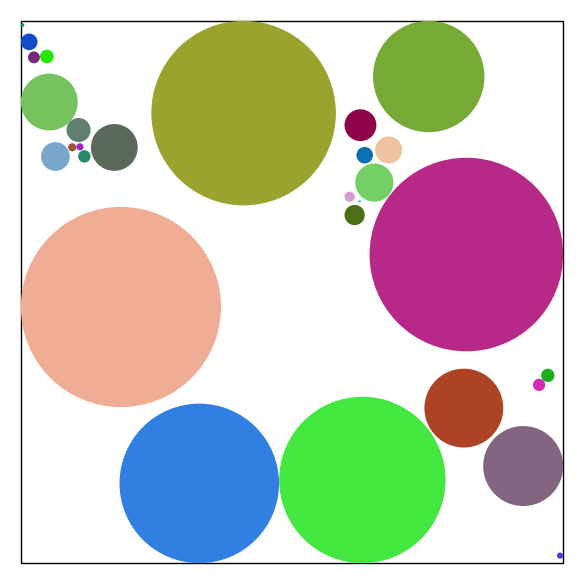
\includegraphics[width=0.5\textwidth]{square_example.png}
%    \end{center}
%}

\subject{Master's Thesis}
\title{Algorithms \\for Circle Packing}
\author{\sffamily\LARGE Sebastian Morr}
\date{\large June 2, 2016}
\publishers{\textbf{Institute of Operating Systems and Computer Networks\\Prof.\,Dr.\,Sándor\,Fekete}\\
\vspace*{2em}
Supervisors:\\
Dr.\,Christian\,Scheffer\\
Jan-Marc\,Reinhardt,\,M.\,Sc.}

\begin{document}

%\frontmatter % roman page numbering

\maketitle
\cleardoublepage

% statement of originality
\thispagestyle{plain} % no header
\vspace*{7cm}
\centerline{\bfseries Statement of Originality}
\vspace*{1em}
\noindent
This thesis has been performed independently with the support of my supervisors.
To the best of the author's knowledge, this thesis contains no material previously
published or written by another person except where due reference is made in the text.

\par
  \bigskip\noindent Braunschweig, June 2, 2016 \par
  \vspace*{10mm}
  \hfill\hrulefill
\cleardoublepage

% abstract
\thispagestyle{plain} % no header
\centerline{\bfseries Abstract}
\vspace*{1em}
\noindent
Very abstract indeed.
\cleardoublepage

\section*{Acknowledgments}

I would like to thank the following people for their support in the creation of this thesis:

\section*{Colophon}

This document was created using \LaTeXe\ by Leslie Lamport and contributors, and \KOMAScript\ by Frank Neukam, Markus Kohm, and Axel Kielhorn. The figures were created using PGFPlots by Christian Feuersänger and Ti\textit{k}Z by Till Tantau. The text is set in the Latin Modern font family by Bogusław Jackowski, Janusz M. Nowacki and Marcin Woliński, the monospaced font is \texttt{Bera Mono}, based on Bitstream Vera.

\cleardoublepage
\setcounter{tocdepth}{2}

\tableofcontents
\cleardoublepage

%\listoffigures
%\cleardoublepage
%
%\listoftables
%\cleardoublepage

\mainmatter % arabic numbering

\chapter{Introduction}

%\begin{figure}[htbp!]
%    \centering
%
%    \begin{tikzpicture}[scale=2.5]
%        \squareworstcase
%    \end{tikzpicture}
%
%    \caption{Worst-case instance for packing density?}
%    \label{fig:worst-case}
%\end{figure}
%
%Consider the circle packing shown in \Cref{fig:worst-case}. For these two circles, the surrounding square is the smallest one in which the circles can be packed. Originally, we considered the following problem: Does this instance constitute the worst case in terms of packing density, or is there a set of circles with the same combined area that cannot be packed into this square? Put differently, can all other sets of circles with the same combined area as these two
%(like the one in \Cref{fig:big-question})
%be packed into this specific square?
%We will give a constructive proof that this is indeed the case.
%
%\begin{figure}[htbp!]
%    \centering
%
%    \begin{tikzpicture}[scale=2.5]
%        \bigquestion
%    \end{tikzpicture}
%
%    \caption{Can these circles be packed?}
%    \label{fig:big-question}
%\end{figure}

%Furthermore, we will describe an algorithm which is able to pack circles into non-acute triangles with worst-case density.

\section{Results}

We give a constructive proof that all circle instances with a combined area of $a$ can be packed into all non-acute triangles with an incircle not larger than $a$.

Furthermore, ...

\section{Related work}

Packing objects into a container is a classic, intuitive problem...

Most works concerned with circle packing follow one of the two following approaches:

Either they model the packing problem as an optimization problem, and solve it using commercial nonlinear solvers.

Or they apply heuristics.

In this thesis, we are interested in approximation algorithms, which give certain performance guarantees on the obtained results.

\paragraph{History}

The packing of equal circles in a square has received particular attention in the past.

The optimal packings of up to nine equal circles were already proven in 1965.
\textcite{schaer1965densest} proofed the optimal solutions for $n = 7$ and $n = 8$, and \textcite{SM1965geometric} the one for $n = 9$.
The optimal solution for $n = 10$ was not confirmed until 1990 by \textcite{DPW1990optimal}. In the same paper, optimal solutions for 11, 12 and 13 circles were also proven.
See \textcite{WMP1994history} for an overview of the history of optimal solutions for $n \le 13$.

The best known solutions for packing equal circles into squares, circles, rectangles, and other containers are continuously published on \url{packomania.com} \cite{specht2015packomania}.

\paragraph{Global optimization}

\textcite{GJLS2009solving} also model the problem of packing circles into a circle as a global nonlinear optimization problem and apply a method similar to Multistart, which they refer to as \emph{Monotonic Basin Hopping}.

\paragraph{Unequal circles in squares}

The problem of finding the smallest square that suffices for packing any set of circles of total area 1 was posed by \textcite{DFL2010circle}. They described a quadtree-based approximation scheme which could guarantee a packing density of $\pi/16 \approx 0.196349$.


\paragraph{Equal circles in circle}

\textcite{lubachevsky1997curved} studied \emph{curved hexagonal packings} of equal circles in a circle, a pattern derived from known best packings of circles in hexagons. For large $n$, a curved hexagonal packing was found to be not optimal. Instead, good packings found by the authors seemed to have a curved hexagonal-packed core and an irregular pattern along the periphery.

\paragraph{Unequal circles in circle}

\textcite{WHZX2002improved} describe a “quasi-physical, quasi-human” approach, which first simulates the circles according to gravity and then finds circles which are "most squeezed", and re-insert them randomly.

\textcite{BG2010new} note that, given the contacts of the circle objects to the containers boundary beforehand, the numer of constraints is reduced significantly. They learn this information from previously best known solutions in the literature and solve the now overdetermined linear system to get high-precision results.

\paragraph{Circles in strips}

\paragraph{Improvement steps}

\textcitr{SY2004mathematical} formulate a method of transitioning from one local optimum to a better one when packing unequal circles into a strip, based on a reduced gradient method.

\paragraph{Maximum packing densities}

Thue's proof is generally considered incomplete, and was first fixed by L. F. Toth 1940 TODO. For a simple, short proof see \cite{CW2010simple}.

\paragraph{Hardness}

Packing arbitrary objects into arbitrary containers can immediately shown to be NP-hard by reduction from \textsc{2-PARTITION}.

But also for similar objects and arbitrary containers \textcite{FPT1981optimal} showed this problem to be NP-hard by a reduction from \textsc{3-SAT}. They constructed gadgets for variables and clauses and connected them with wires.

The decision problem whether it is possible to pack a given set of squares into a square container was shown to be strongly NP-complete by \textcite{LTWYC1990packing} through a reduction from \textsc{3-PARTITION}.

The decision problem whether it is possible to pack a given set of unequal circles into a square or an equilateral triangle was shown to be NP-complete by \textcite{DFL2010circle}.

\subsection{Packing squares}

Approximation algorithms which pack squares are interesting in this context as we can directly use them for packing circles: We simply embed each circle with radius $r$ in a square of edge length $2r$.

This means that if we are given an algorithm which can pack all square instances with a total area of $a$ into a given shape, we immediately get an algorithm which can pack all circle instances with a total area of $\frac{\pi}{4}a$.

\paragraph{Packing squares into a rectangle}

\textcite{MM1967some} developed an algorithm which can pack all square instances with a total area of $1/2$ into the unit square.
%proved a critical density of $\nicefrac{1}{2}$ when packing squares into a square.
They sort the squares by their size and place them into the square in a shelf-like manner, see fig TODO.
They also proofed that $1/2$ is the critical density for packing squares into a square: Two squares, each with an area of more than $1/4$ of the container's area, cannot be packed, see fig TODO.
As by above remark, their algorithm can also be used to pack circles: It can pack all circle instances with a total area of $\frac{\pi}{8} \approx 0.39269908$ into the unit square.

\textcite{KK1975optimal} showed that any square instance of total area 1 can be packed into a rectangle of dimensions $2/\sqrt{3}$ times $\sqrt{2}$, and that this is the smallest-area rectangle with that property. The packing density in this case is 0.612372435695. Applied to circles, this result means that all circle instances with a total area of 1 can be packed into a rectangle of dimensions $4/\sqrt{3\pi}$ times $2\sqrt{2}/\sqrt{\pi}$.

\textcite{hougardy2011packing} showed that for any set of squares with a total area of 1, there is some rectangle with an area $< 1.4$ in which the squares can be packed using a computer generated proof.

%Online
%Upper bound:
%Lower bound:

\paragraph{Heuristics}

As one of the first to consider the packing of unequal circles into rectangles, \textcite{GGL1995packing} developed a set of heuristics, based on enumerating \emph{stable} solutions, where a circle is either on the ground or has two lower contacts. To get out of local optima, they apply a variety of approaches, like “shaking down” circles or apply genetic algorithms to improve the stable solutions.

\textcite{HLLX2006new} apply a quasi-human heuristic, which places new circles in gaps of approximately the same size as the circle, and combine it with a self look-ahead strategy which evalutates how beneficial the coice of a certain placement for each circle is.

\textcite{LIE2014approximate} compute approximated solutions to packing circles into rectangles by restricting their coordinates to a regular grid and formulate a binary LP, where the variables represent the assignment of the centers to the grid nodes.

\textcite{ZYC2015packing} extend the GVS to allow packing into \emph{damaged squares}, squares with some smaller squares removed from it. They enhance the GVS by Simulated Annealing and get significantly better results in their experiments compared to GVS.

\textcite{ZD2005effective} combine simulated annealing and tabu search to pack unequal circles into a circle.

\textcite{GLNO1998dense} propose a \emph{billiard simulation}, in which the circles are physically simulated as hard disks, and apply some additional steps to tighten the found packings.

\paragraph{Unsorted}

\textcite{MPSSW2014polynomial} devised a general polynomial-time approximation schemes for packing circle-like objects into containers, which first packs a constant number of large objects, and then fills up the unused space with the small objects.

\textcite{HMS2016bounded} devised an asymptotic approximation algorithm, which can pack unequal circles into square bins in an online fashion with an asymptotic competitive ratio of at most 2.4394. They also gave a lower bound of 2.2920 for any online bounded space algorithm for that problem. The algorithm packs large circles according to the best known packings of equal circles and puts small circles into recursively subdivided hexagonal bins.

\section{Applications}

Circle packing has all kinds of useful applications in engineering, science and everyday life.

% categories: coverage, storage, packaging, tree exploitation, cutting industry

Running optical fibers through a tube or placing many differently-sized pipes through a smaller one \parencite{WHZX2002improved}

For example, car manufacturers may want to drill circular holes into a car's body to route a number of sensor cables through that hole, but keep the hole as small as possible not to weaken the car's body \cite{SSSKK2004disk}.

Placing radio towers for maximal coverage \parencite{SMCSCG2007new}.

Cutting circular pieces from a material, minimizing waste, loading a container (like a vehicle or a parcel with cylindrical objects, minimizing the number of nodes in a geographical communication network or dispersing facilities so that the minimum distance between any two is maximized, the layout of control panels containing circular controls (like in airplanes) \parencite{CKP2008solving}

Other applications stem from chemistry, where one can study dense packing of atoms in crystals or macromolecules \cite{WMP1994history}.
% or info processing (sperical codes)
%https://en.wikipedia.org/wiki/Quadrature_amplitude_modulation

Photo collage "Content-aware photo
collage using circle packing"

Cutting a given set of disks from a piece of material, while wasting as little as possible of it \cite{SMCSCG2007new}

Foresting, where one wants to plant trees so that the forest will be as dense as possible, but the trees do not hinder each other's growth \cite{SMCSCG2007new}.

%storage of a cylindrical drums into containers or
%stocking them into an open area, packaging bottles or cans into the smallest box,

%"Other applications one can find in the motor
%cycle industry, communication networks, facility location and
%dashboard layout"

Another application includes the design of crease patterns for Origami, where one wants to find a sequence of folds of a square piece of paper, so that the result resembles a specific shape. This kind of Origami design was pioneered by \cite{lang1996computational}. Using circle packings, one can find crease patterns for arbitrary stars.

%\chapter{Preliminaries}

\section{Circle instances}

We start off with some definitions which make our life easier when talking about circle instances:

\begin{definition}
    For each $0 \le a$, an \emph{$a$-circle} is a circle with an area of $a$.
\end{definition}

\begin{definition}
    A \emph{circle instance} is a multiset of non-negative real numbers, which define the circles' areas. Addition of circle instances is defined like on multisets.
    For any circle instance $C$, $\mysum(C)$ is the combined area of the instance's circles and $\min(C)$ is the area of the smallest circle contained in the instance.
\end{definition}

For example, for the circle instance $C = \{3,2,1,4\}$, $\mysum(C) = 10$ and $\min(C) = 1$.

\begin{definition}
    $\C$ is the set of all circle instances. $\C(a)$ consist of exactly those circle instances $C$ with $\mysum(C) \le a$. Finally, $\C(a,b)$ consists of exactly those circle instances $C \in \C(a)$ with $\min(C) \ge b$.
\end{definition}

\section{Shapes}

\begin{definition}
    A shape's \emph{incircle} is the largest circle that can be packed into the shape.
\end{definition}

\begin{definition}
    A shape's \emph{twincircles} are the maximum-area circle instance consisting of exactly two equal circles that can be packed into the shape. The shape's \emph{twincircle area} is their combined area.
\end{definition}

\section{Packing}

\begin{definition}
    A \emph{packing} of a circle instance $C$ into a shape $s$ is...
\end{definition}

%\chapter{General techniques}

\section{Greedy splitting}

The core idea of the proposed packing algorithms is to recursively split the set of input circles into groups. The method which performs this splitting resembles a greedy scheduling algorithm. It is going to be important for the packing algorithm that the ratios of the groups' sums is close to certain factors.

The algorithm, \textsc{Split}, takes two parameters: The first is an arbitrary circle instance $C$. The second is a tuple of positive factors, which determines which percentages of $C$'s sum should go into the respective groups. For example, if we wanted to split $C$ into equally sized halves, we could choose the tuple $(1,1)$, and if we wanted to split $C$ into four groups with the proportions 1:1:3:3, we could use $(1,1,3,3)$. We call this tuple the \emph{split key}:

\begin{definition}
    A \emph{split key} is a tuple of at least two positive real numbers.
\end{definition}

In each step, \textsc{Split} adds the largest remaining circle of the input instance to the “emptiest” group---the group where the ratio between the current sum and the associated factor of the split key is the smallest. The scenario which is easiest to imagine is when the split key actually describes the desired total area of that group, and \textsc{Split} puts the next circle into the group which has the smallest “filling level”.

\begin{algorithm}[htbp!]
    \caption{\textsc{Split}$(C,F)$}
    \begin{algorithmic}
        \Require A circle instance $C$ and a split key $F = (f_1, f_2, \dots, f_n)$
        \Ensure Circle instances $C_1, C_2, \dots, C_n$
        \For{$i = 1$ to $n$}
            \State $C_i \gets \emptyset$
        \EndFor
        \State Sort $C$ descending by size
        \ForAll{$c \in C$}
            \State $j = \argmin_{i} \frac{\mysum(C_i)}{f_i}$\Comment{Find the index of the emptiest instance}
            \State $C_j \gets C_j \cup \{c\}$
        \EndFor
    \end{algorithmic}
\end{algorithm}

Of course, it will not always be possible to achieve these desired ratios exactly (for example if the input instance consists of few very large elements which cannot be distributed in the specified ratios), but we can derive an interesting property from the resulting subinstances if the resulting group's sizes derive from the split key:

\begin{lemma}\label{th:split-property}
    For any circle instance $C$ and any split key $F = (f_1, f_2, \dots, f_n)$, \textsc{Split}$(C,F)$ decomposes $C$ into circle instances $C_1$, $C_2$, $\dots$, $C_n$.
    Set $a_i \coloneqq \mysum(C_i)$ and $r \coloneqq \min\{\frac{a_1}{f_1}, \frac{a_2}{f_2}, \dots, \frac{a_n}{f_n}\}$.
    Then $\min(C_i) \ge a_i - f_i r$ for each $1 \le i \le n$.
\end{lemma}

\begin{proof}
    For the minimum size, assume for contradicion that $C_i$ contained an element smaller than $a_i - f_i r$. All elements which were put into $C_i$ after that have to be at least as small, as the elements were inserted by descending size. So the last element put into $C_i$ (let us call it $c$) would be smaller than $a_i - f_i r$, as well.
    But this means that $\frac{a_i - c}{f_i} > \frac{a_i - (a_i - f_i r)}{f_i} = r$, meaning that at the moment before $c$ was inserted, the relative filling level of $C_i$ would already have been larger than $r$. But $r$ is the smallest relative filling level by the time the algorithm ends, so at the time when $c$ is inserted, the group's filling level would have been at least as small.
    This is a contradiction to the algorithm's greedy nature, as \textsc{Split} would not have but $c$ into the (fuller) group $C_i$ in this situation.
\end{proof}

%Here is a definition that makes it easier to talk about 
%The next definition looks a bit weird, but makes it easier to talk about multiple shapes:
To make it easier to talk about the properties of the groups output by \textsc{Split}, we introduce the notion of \emph{$(F,b)$-roundedness}:

%\begin{definition}\label{def:rounded}
%    For any split key $F$ of length $n$, we say that a tuple of $n$ shapes is \emph{$(F,b)$-rounded}, if the $i$-th shape is a $\C(a_i, \min\{b,a_i - f_i r\})$-shape, with $r = \max\{\frac{a_i}{f_i}|i \in 1,2,\dots,n\}$.
%\end{definition}

\begin{definition}\label{def:rounded}
    For any split key $F = (f_1, f_2, \dots, f_n)$ and any $b \ge 0$ we say that $n$ tuples $(a_1, b_1)$, $(a_2, b_2)$, $\dots$, $(a_n, b_n)$ are \emph{$(F,b)$-rounded} if each $b_i = \max\{b,a_i - f_i \min\{\frac{a_1}{f_1}, \frac{a_2}{f_2}, \dots, \frac{a_n}{f_n}\}\}$.
\end{definition}

We can now associate this property with \textsc{Split} in the following theorem:

\begin{theorem}\label{th:split-sets}
    For any $C \in \C(a,b)$, and any split key $F = (f_1, f_2, \dots, f_n)$, \textsc{Split}$(C,F)$ produces $n$ subinstances $C_1 \in \C(a_1, b_1), C_2 \in \C(a_2, b_2), \dots, C_n \in \C(a_n, b_n)$, so that $C_1 + C_2 + \dots + C_n = C$ and the instance sets' parameters are $(F,b)$-rounded.
\end{theorem}

\begin{proof}
    That the subinstances add up to the original instance is obvious from the algorithm.
    For the roundedness, as $\min(C) \ge b$, the subinstances must have the same property. Additionally, by \Cref{th:split-property}, $C_i \in \C(a_i, a_i - f_i \min\{\frac{a_1}{f_1}, \frac{a_2}{f_2}, \dots, \frac{a_n}{f_n}\})$. Thus, the subinstances satisfy \Cref{def:rounded}.
\end{proof}

%What is means for shapes to be $(F,b)$-rounded is that we lift some requirements on which instances they need to be able to pack. We combine two lower bounds for the minimum size of the instances: First, the shapes never need to be able to pack any instances containing circles smaller than $b$. Second, they reflect the \textsc{Split}-algorithm's minimum element sizes stated in \Cref{th:split-property}. If a subinstance $C_i$ returned by \textsc{Split} can not possibly contain any circles smaller than a certain size, it makes sense to also relax the requirements for the shapes in which these subinstances will be packed: It suffices if they can pack those instances where the circles have this minimum size. Whichever of the two circle sizes requirements is largest, determines the “minimum size” of the rounded shape.

%Put differently, to have $F$-rounded shapes of the correct totals is a sufficient condition to be able to pack resulting subinstances of a \textsc{Split} operation into them. This is expressed in the following lemma:

\section{Shapes, Rounding, and Split Packing}

%We will now make some general observations about shapes which are suitable to pack certain classes of circle instances. Most of the proofs appearing in later chapters, while tailored to specific kinds of shapes (triangles, squares), will use these quite universal theorems.
We will now turn to general shapes. It is often interesting to state that a shape can pack certain classes of circle instances. For this, we define the term \emph{$\mathcal{C}$-shape}:

\begin{definition}
    For any $\mathcal{C} \subseteq \C$, a $\mathcal{C}$-shape is a shape in which each $C \in \mathcal{C}$ can be packed.
\end{definition}

For example, if a shape is a $\C(a)$-shape, it means that each circle instance with a sum of $a$ can be packed into the shape. That's an interesting property that we will hunt after for most of this thesis, as it means no matter how the instances divide the area $a$ into circles, they can all be packed into the shape.

For convenience, we define the \emph{sum} of a $\C(a)$-shape:

\begin{definition}
    For a $\C(a)$-shape, we call $a$ the shape's \emph{sum}.
\end{definition}

We also extend our roundedness definition to shapes:

\begin{definition}
    We say that $n$ shapes are $(F,b)$-rounded if they are a $\C(a_1, b_1)$-shape, a $\C(a_2, b_2)$-shape, \dots, and a $\C(a_n, b_n)$-shape and their parameter tuples are $(F,b)$-rounded.
\end{definition}

%Recall that $\C(a,b)$ contains all circle instances with a sum of $a$ and a minimum circle size of $b$. If a shape is a $\C(a,b)$-shape with $b > 0$, it means that it can pack all circle instances $C$ with $\mysum(C) \le a$ and $\min(C) \ge b$. This leads to an interesting effect: As the shape does not need to accomodate for circles smaller than $b$, it can be “rounded” to a radius of a $b$-circle. Sharper corners will be superfluous, as circles in $\C(a,b$) will not be permitted to be placed there anyway.
%In particular, this means that the shape's maximum local curvature can be the curvature of a $b$-circle, as when the curvature is 


%\begin{theorem}
%    A shape is a $\mathcal{C}$-shape, if, for a given decomposition method, for all possible decompositions $C_1, C_2, \dots, C_n$ of any $C \in \mathcal{C}$, one can always find $n$ shapes in which the resulting subinstances can be packed, and which fit into the original shape.
%\end{theorem}

%\begin{theorem}
%    A shape is a $\C(a,b)$-shape, if there is a split key $F$, so that for all $a_1 + a_2 + \dots + a_n \le a$, one can find a $\C(a_1)$-shape, a $\C(a_2)$-shape, \dots, and a $\C(a_n)$-shape, which are $F$-rounded and fit into the original shape.
%\end{theorem}

%\begin{lemma}\label{th:split-rounded}
%    Given an arbitrary $C \in \C(a,b)$ and a split key $F$, use \textsc{Split}$(C,F)$ to decompose $C$ into $n$ subinstances. Call the subinstances' totals $a_1$, $a_2$, \dots, $a_n$. If we can find a $\C(a_1, b_1)$-shape, a $\C(a_2, b_2)$-shape, \dots, and a $\C(a_n, b_n)$-shape, so that the shapes' parameters are $(F,b)$-rounded, we can pack $C$ into the shapes.
%\end{lemma}
%
%\begin{proof}
%    We know from \Cref{th:split-sets} that \textsc{Split} only produces subinstances $C_i \in \C(a_i, b_i)$ so that the instance set's parameters are $(F,b)$-rounded. As the $i$-th shape is a $\C(a_i, b_i)$ shape, we can pack $C_i$ into it.
%\end{proof}

With these preparations, we can now state our central \emph{split packing} theorem:

\begin{theorem}[Split Packing]\label{th:splitpack}
    For a given shape $s$, and for any $0 \le b < a$, if there is a split key $F$ of length $n$, so that for all tuples $(a_1, a_2, \dots, a_n)$ with $a_1 + a_2 + \dots + a_n \le a$
    one can find $n$ $(F,b)$-rounded shapes of matching sums,
    and these shapes can be packed into $s$, then $s$ is a $\C(a,b)$-shape.
\end{theorem}

\begin{proof}
    Consider an arbitrary $C \in \C(a,b)$. Regardless of which groups \textsc{Split} produces, we know from \Cref{th:split-sets} that they always are elements of $(F,b)$-rounded circle instance sets.
    As we can find $(F,b)$-rounded shapes with matching sums, the $i$-th group can be packed into the $i$-th shape.
    As these shapes also fit into $s$, we know that we can pack $C$ into $s$.
\end{proof}

As this theorem is important for the whole thesis, let us rephrase it: \Cref{th:splitpack} describes what is sufficient to proof that a shape is a $\C(a,b)$-shape: Find a shape-specific split key $F$ and show that for all possible decompositions of the area $a$ (which is going to be perfomed by \textsc{Split}), that one can find $(F,b)$-rounded shapes of matching sums that fit into the original shape.

The general \textsc{Splitpack} algorithm, then, reads as follows:

\begin{algorithm}[htbp!]
    \caption{\textsc{Splitpack}$(s,C)$}
    \begin{algorithmic}
        \Require A $\C(a,b)$-shape $s$ and a circle instance $C \in \C(a,b)$
        \Ensure A packing of $C$ into $s$
        \State Determine split key $F$ for $s$
        \State $(C_1, C_2, \dots, C_n) \gets \textsc{Split}(C,F)$
        \State $(s_1, s_2, \dots, s_n) \gets$ any $(F,b)$-rounded shapes with $\mysum(s_i) = \mysum(C_i)$
        \State Pack these shapes into $s$
        \ForAll{$C_i \in (C_1, C_2, \dots, C_n)$}
            \State \Call{Splitpack}{$s_i, C_i$}
        \EndFor
    \end{algorithmic}
\end{algorithm}

%One needs the following elements to use \textsc{Splitpack} for a shape:
%
%\begin{enumerate}
%    \item A strategy to determine the split factor $F$
%    \item A strategy to determine $n$ $(F,b)$-rounded shapes of matching sums for each decomposition of the area $a$
%    \item A strategy to pack these shapes into $s$
%\end{enumerate}
%
%To proof that the shape is indeed a $\C(a,b)$-shape, one needs to show that these three strategies always work.

%\section{Normalization}

%In some proofs, we will normalize the instances, shapes, or figures in question. For example, we can scale all areas involved up by a factor of $f$, as long as we scale all lengths up by a factor of $\sqrt{f}$.

\section{Approximation factor}

For equal circles, we get an approximation factor of...

%\chapter{Triangular containers}

\section{Hats}

We turn to specific classes of container shapes now. For each shape, we are going to proof the \emph{worst-case packing density}. In each case, we are going to give a circle instance with total area $a$ and show two properties: First, that for all $a' > a$, there are circle instances of total area $a'$ which \emph{cannot} be packed. Second, that all instances of total area $a$ can be packed.

The respective worst-case instances for all container classes are depicted in Fig TODO.

A useful family of shapes, which can be packed into each other quite well, are rounded, non-acute triangles. We call these shapes \emph{hats}:

\begin{definition}
    For each $0 \le b \le a$, an \emph{$(a,b)$-hat} is a non-acute triangle with an incircle of area $a$, whose corners are rounded to the radius of a $b$-circle, see \Cref{fig:hat}. Call the triangle's longest side the hat's \emph{base}, and the triangle's angles to the left and to the right of the base the triangle's \emph{right-angle} and \emph{left-angle}.
    %An $a$-hat is an $(a,0)$-hat.
    If we say \emph{right hat} or \emph{obtuse hat}, the hat is based on a right/obtuse triangle.
\end{definition}

\begin{figure}[htbp!]
    \centering

    \begin{tikzpicture}[scale=3]
        \hatsimple{\defaulta}{\defaultb}{\defaultr}
    \end{tikzpicture}

    \caption{An $(a,b)$-hat.}
    \label{fig:hat}
\end{figure}

\begin{definition}\label{def:hat-split-key}
    A hat's \emph{associated split key} equals the tuple of the areas of the two circles incribed in the hat's two sides when splitting the underlying triangle orthogonally to its base through its tip, see \Cref{fig:hatf}.
\end{definition}

\begin{figure}[htbp!]
    \centering

    \begin{tikzpicture}[scale=3]
        \hatf{\defaulta}{\defaultb}{\defaultr}
    \end{tikzpicture}

    \caption{A hat's \emph{associated split key} equals $(f_1, f_2)$}
    \label{fig:hatf}
\end{figure}

%%For the following proofs, we need to know a hat's dimensions in detail. We construct these measures using \Cref{fig:construction}.
%%
%%\begin{lemma}\label{lm:sizes}
%%    Let $r$ be the radius of an $a$-circle, and $s$ be the radius of a $b$-circle.
%%
%%    A ($a,b$)-hat has
%%    \begin{itemize}
%%        \item height $h(a) = \textcolor{blue}{r + r\s} = \sqrt{\frac a \pi}(1+\s)$,
%%        \item width $w(a,b) = 2\textcolor{blue}{(r+r\s)} - 2\textcolor{orange}{s\s} = \sqrt{\frac a \pi}(2+2\s)-\sqrt{\frac b \pi}2\s$,
%%        \item and diagonal $d(a,b) = \textcolor{red}{(r+r\s)\s} - \textcolor{orange}{s\s} = \sqrt{\frac a \pi}(2+\s)-\sqrt{\frac b \pi}\s$.
%%    \end{itemize}
%%
%%    We define two additional measures for the case when one of the corners is not rounded:
%%    \begin{itemize}
%%        \item corner-width $w'(a,b) = w(a,b) + \textcolor{orange}{s\s} = \sqrt{\frac a \pi}(2+2\s)-\sqrt{\frac b \pi}\s$,
%%        \item and corner-diagonal $d'(a) = d(a,0) = \sqrt{\frac a \pi}(2+\s)$.
%%    \end{itemize}
%%\end{lemma}
%%
%%\begin{figure}[htbp!]
%%    \centering
%%
%%    \begin{tikzpicture}[scale=4]
%%        \hatconstruction
%%    \end{tikzpicture}
%%
%%    \caption{Constructing the dimensions of an $(a,b)$-hat.}
%%    \label{fig:construction}
%%\end{figure}
%%

\begin{lemma}\label{th:hatsinhat}
    Consider an $(a,0)$-hat with the associated split key $F = (f_1, f_2)$, and call its left- and right-angles $\alpha$ and $\beta$.
    For all $(F,0)$-rounded tuples $(a_1, b_1)$ and $(a_2, b_2)$ with $a_1 + a_2 \le a$, the following two shapes can be packed into the hat:
    \begin{itemize}
        \item A right $(a_1,b_1)$-hat with a right-angle of $\alpha$ and
        \item a right $(a_2,b_2)$-hat with a left-angle of $\beta$.
    \end{itemize}
\end{lemma}

\begin{proof}
    Place the hats' tips at the bottom of the container hat, rotate their $\alpha$- and $\beta$-angles towards the container's matching angles and push them as far to the left/right as possible. Figure \Cref{fig:hatsinhat} shows examples how this packing looks like for different values of $a_1$ and $a_2$.

    \begin{figure}[htbp!]
        \centering

        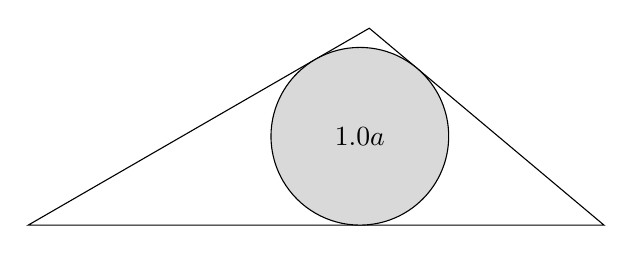
\begin{tikzpicture}[scale=2]
            \hatsinhat{\defaulta}{\defaultb}{0}{0}
        \end{tikzpicture}
        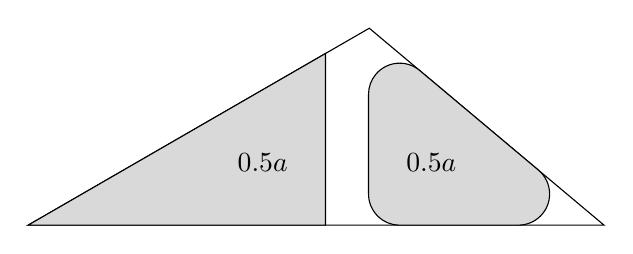
\begin{tikzpicture}[scale=2]
            \hatsinhat{\defaulta}{\defaultb}{0.5}{0}
        \end{tikzpicture}

        \vspace{2mm}

        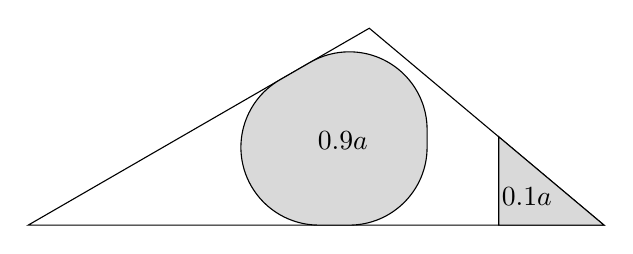
\begin{tikzpicture}[scale=2]
            \hatsinhat{\defaulta}{\defaultb}{0.1}{0}
        \end{tikzpicture}
        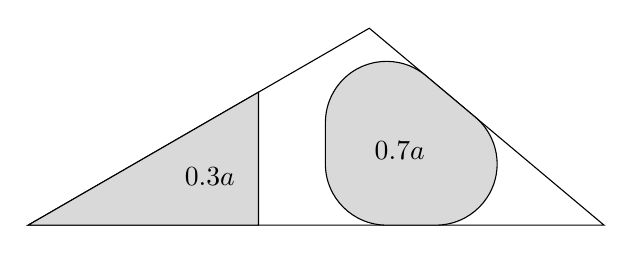
\begin{tikzpicture}[scale=2]
            \hatsinhat{\defaulta}{\defaultb}{0.7}{0}
        \end{tikzpicture}

        \vspace{2mm}

        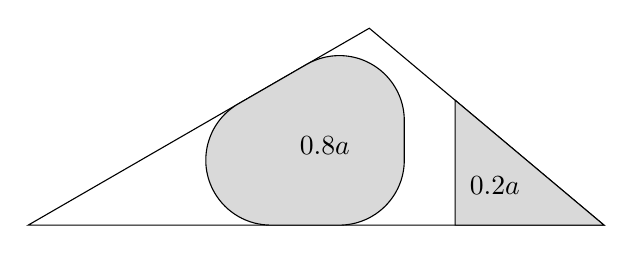
\begin{tikzpicture}[scale=2]
            \hatsinhat{\defaulta}{\defaultb}{0.2}{0}
        \end{tikzpicture}
        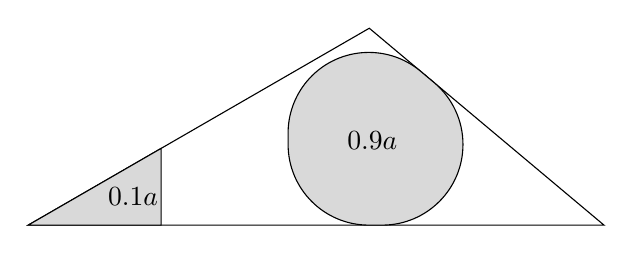
\begin{tikzpicture}[scale=2]
            \hatsinhat{\defaulta}{\defaultb}{0.9}{0}
        \end{tikzpicture}

        \vspace{2mm}

        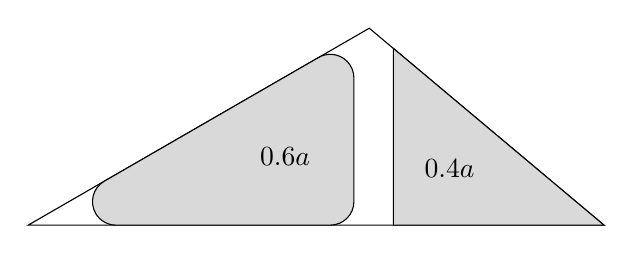
\begin{tikzpicture}[scale=2]
            \hatsinhat{\defaulta}{\defaultb}{0.4}{0}
        \end{tikzpicture}
        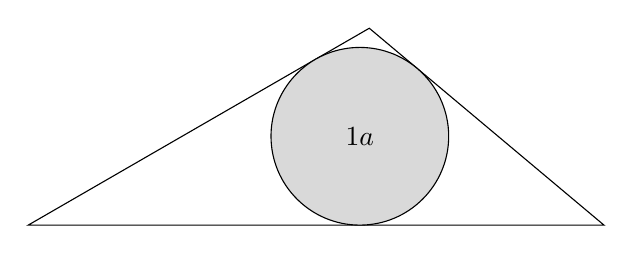
\begin{tikzpicture}[scale=2]
            \hatsinhat{\defaulta}{\defaultb}{1}{0}
        \end{tikzpicture}

        \caption{Hat-in-hat packings for different values of $a_1$ and $a_2$}
        \label{fig:hatsinhat}
    \end{figure}

    This placement constitutes a valid packing if (1) the hats do not overlap each other and (2) the hats fit into the hat individually. We are going to proof these two properties separately.

    \begin{itemize}
        \item[(1)]
            We want to show that the hats do not overlap each other.

            We first normalize the container hat's width to 1 and make an observation about the partial widths $l$ and $r$ in \Cref{fig:hatlr}: If the top angle is a right angle, the partial widths have the same lengths as the triangle's two cathetus $x$ and $y$ (TODO is it clear why?), so by Pythagoras, $l^2 + r^2 = 1$. If the top angle is more obtuse, but the incircle's center stays at the same $x$-coordinate (like the dotted variant), both $l$ and $r$ shrink, so for each hat, $l^2 + r^2 \le 1$, or $r \le \sqrt{1-l^2}$.

            \begin{figure}[htbp!]
                \centering

                \begin{tikzpicture}[scale=3]
                    \hatlr{\defaulta}{\defaultb}{39}{51}
                \end{tikzpicture}

                \caption{$l^2 + r^2 \le 1$ holds for each non-acute triangle}
                \label{fig:hatlr}
            \end{figure}

            The two hats do not overlap if their incircles do not overlap. If we enclose their incircles with hats which are \emph{similar} to the container, like in \Cref{fig:hatsoverlap}, we see that they do not overlap if the following condition holds:

            \begin{equation}\label{eq:trifit}
                lf + rg \le w
            \end{equation}

            \begin{figure}[htbp!]
                \centering

                \begin{tikzpicture}[scale=3]
                    \hatsoverlap{\defaulta}{\defaultb}{\defaultx}{0}
                \end{tikzpicture}

                \caption{$f^2 + g^2 \le w^2$ for each non-acute triangle}
                \label{fig:hatsoverlap}
            \end{figure}

            Also note that for similar hats, the ratio between their incircle's area and the square of their widths is constant (TODO clear why?). This means that if $a_1 + a_2 \le a$, then $f^2 + g^2 \le w^2$. Thus, $g \le \sqrt{w^2-f^2}$.

            Putting it all together, we can show that \Cref{eq:trifit} is true:

            \begin{align*}
                lf + rg
                &\le lf + \sqrt{1-l^2} \sqrt{w^2-f^2}\\
                &= lf + \sqrt{(1-l^2)(w^2-f^2)}\\
                &= lf + \sqrt{w - \textcolor{blue}{l^2w^2} - \textcolor{blue}{f^2} + l^2f^2}\\
                &\le lf + \sqrt{w - \textcolor{orange}{2lwf} + l^2f^2}\addtocounter{equation}{1}\tag{\theequation}\label{eq:am-gm}\\
                &= lf + \sqrt{(w-lf)^2}\\
                &= w
            \end{align*}

            Line \ref{eq:am-gm} is a consequence of the inequality of arithmetic and geometric means: $\frac{lw+f}{2} \ge \sqrt{lwf} \Rightarrow \frac{(lw+f)^2}{4} \ge lwf \Rightarrow l^2w^2 + 2 lwf + f^2 \ge 4 lwf \Rightarrow \textcolor{blue}{l^2w^2 + f^2} \ge \textcolor{orange}{2lwf}$.

        \item[(2)]
            It is left to show that the hats fit inside the container individually.

            If a hat's incircle is not larger than the incircle of the container hat's side, it will fit inside without question (like all the non-rounded hats in \Cref{fig:hatsinhat}).

            So let us assume $a_i > f_i$. For this proof, normalize the container hat's incircle to 1. Again, for hats similar to the container hat's right side, the ratio between the square root of its incircle's area and the length of its base is constant. We call this constant $d$.
            %Also, we are interested in the fraction $\frac{x}{d}$ in \Cref{fig:hatpokef}, which specifies “which fraction of the longest side of a triangle similar to the container's right side is above a tangent to its incircle parallel to the container triangle's left side”. We can observe that
            We are also interested in the ratio between the square root of the area of the incircle of a triangle similar to the container triangle and the length of its right side. We call this ratio $e$. See \Cref{fig:hatpokef} for an illustration of $d$ and $e$.

            \begin{figure}[htbp!]
                \centering

                \begin{tikzpicture}[scale=3]
                    \hatpokef{\defaulta}{\defaultb}{\defaultx}{0}
                \end{tikzpicture}

                \caption{The ratios $d$ and $e$ are constant for all similar triangles.}
                \label{fig:hatpokef}
            \end{figure}

            From the same figure we can observe that
            $e\sqrt{a} = d\sqrt{f_i}$, which is equivalent to $e = d\sqrt{\frac{f_i}{a}}$.

            %$$\frac{x}{d} = \frac{d-d\sqrt{f_i})}{d} = 1 - \sqrt{f_i}$$

            In \Cref{fig:hatpoke}, we display the situation when packing a hat into (w.l.o.g.) the right side of the container. $f_i$ is the relevant factor from the split key, $a_i$ is the hat's incircle and $y$ represents the hat's rounding.

            \begin{figure}[htbp!]
                \centering

                \begin{tikzpicture}[scale=3]
                    \hatpoke{\defaulta}{\defaultb}{\defaultx}{0}
                \end{tikzpicture}

                \caption{Various measurements when packing a rounded hat.}
                \label{fig:hatpoke}
            \end{figure}

            The hat is placed in such a way that it will never overlap the bottom or the right side of the containing triangle, so it is sufficient to show that it does not overlap the left side.
            We can tell from \Cref{fig:hatpoke} that this does not happen if the width of the hat's triangle ($d\sqrt{a_i}$), minus the width of the $(y,0)$-triangle similar to the containers right side ($d\sqrt{y}$), plus the length of the right side of the $(y,0)$-triangle similar to the container ($e\sqrt{y}$) is at most the length of the container triangle's right side ($d\sqrt{f_i}$):

            \begin{equation*}
                d\sqrt{a_i} - d\sqrt{y} + e\sqrt{y} \le d\sqrt{f_i}\\
            \end{equation*}

            As observed above, $e = d\sqrt{\frac{f_i}{a}}$ (recall that we normalized $a$ to 1):

            \begin{equation*}
                d\sqrt{a_i} - d\sqrt{y} + d\sqrt{f_i}\sqrt{y} \le d\sqrt{f_i}\\
            \end{equation*}

            We can divide by $d$ and factor out $\sqrt{y}$ to get:

            \begin{equation}\label{eq:tripoke}
                \sqrt{a_i} - (1-\sqrt{f_i})\sqrt{y} \le \sqrt{f_i}
            \end{equation}

            Let $j$ be the index of the other hat to be packed.
            As we normalized $a$ to 1, we know that $a_i + a_j \le 1$. Also, $f_i + f_j \ge 1$ (TODO proof in a not yet existing section about worst cases in acute triangles).

            Since we assumed $a_i > f_i$, $a_i - a_if_i > f_i - a_if_i$ and $\frac{a_i}{f_i} > \frac{1-a_i}{1-f_i} \ge \frac{a_j}{f_j}$ are also true, which means that the relative filling level of group $j$ is lower than that of group $i$.

            So by \Cref{th:split-property}, our hat it is rounded by

            $$y = a_i - f_i\frac{a_j}{f_j} \ge a_i - f_i\frac{1-a_i}{1-f_i} = \frac{a_i(1-f_i)-f_i(1-a_i)}{1-f_i} = \frac{a_i-f_i}{1-f_i}$$

            Insert that into \Cref{eq:tripoke}, and also substitute $f_i = b^2$ and $a_i-f_i = c^2$ to get

            $$\sqrt{b^2+c^2} - (1-b)\frac{c}{\sqrt{1-b^2}} \le b$$

            Bring the subtrahend to the right and square both sides.

            $$b^2+c^2 \le b^2 + \frac{2b(1-b)c}{\sqrt{1-b^2}} + (1-b)^2\frac{c^2}{1-b^2}$$

            Subtract $b^2$ and divide by $c$.

            $$c \le \frac{2b(1-b)}{\sqrt{1-b^2}} + (1-b)^2\frac{c}{1-b^2}$$

            Rearrange,

            $$c\frac{(1-b^2)-(1-b)^2}{1-b^2} \le \frac{(1-b^2)-(1-b)^2}{\sqrt{1-b^2}}$$

            Then multiply with $\sqrt{1-b^2}$:

            $$c\frac{(1-b^2)-(1-b)^2}{\sqrt{1-b^2}} \le \frac{(1-b^2)-(1-b)^2}{\sqrt{1-b^2}}\sqrt{1-b^2}$$

            Divide by the large fraction, and resubstitute:

            \begin{align*}
                &c \le \sqrt{1-b^2}\\
                \iff &c^2 \le 1-b^2\\
                \iff &a_i - f_i \le 1-f_i\\
                \iff &a_i \le 1\\
            \end{align*}

            As $a_i$ is never larger than 1, \Cref{eq:tripoke} is true and the hat always fits into the container.
    \end{itemize}
\end{proof}

In this proof, the container was a $(a,0)$-hat, which is essentially a non-rounded triangle. The next lemma extends this idea to hats which are actually rounded:

\begin{lemma}\label{th:roundedhatsinhat}
    Consider an $(a,b)$-hat with the associated split key $F = (f_1, f_2)$, and call its left- and right-angles $\alpha$ and $\beta$.
    For all $(F,b)$-rounded tuples $(a_1, b_1)$ and $(a_2, b_2)$ with $a_1 + a_2 \le a$, the following two shapes can be packed into the hat:
    \begin{itemize}
        \item A right $(a_1,b_1)$-hat with a right-angle of $\alpha$ and
        \item a right $(a_2,b_2)$-hat with a left-angle of $\beta$.
    \end{itemize}
\end{lemma}

\begin{proof}
    \Cref{th:hatsinhat} tells us that this theorem is true for $b = 0$. Now, the container's corners can be rounded to the radius of a $b$-circle, and we need to show that the two hats from the previous construction still fit inside. But all of the two hat's corners are also rounded to (at least) the same radius, so they will never overlap the container, see \Cref{fig:rounding-hats}.
\end{proof}

\begin{figure}[htbp!]
    \centering

    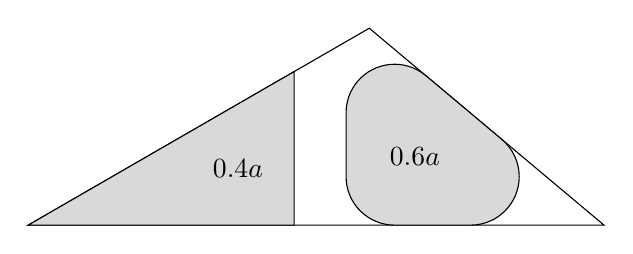
\begin{tikzpicture}[scale=2]
        \hatsinhat{\defaulta}{\defaultb}{\defaultx}{0}
    \end{tikzpicture}
    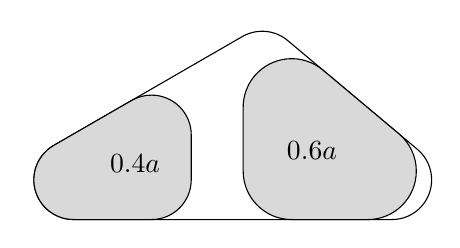
\begin{tikzpicture}[scale=2]
        \hatsinhat{\defaulta}{\defaultb}{\defaultx}{\defaultr}
    \end{tikzpicture}

    \caption{Rounding all hats' corners by the same radius does not affect the packing.}
    \label{fig:rounding-hats}
\end{figure}

\begin{theorem}\label{th:hats}
    Each $(a,b)$-hat is a $\C(a,b)$-shape.
\end{theorem}

\begin{proof}
    %\Cref{def:hat-split-key} tells us how to compute the split key $F$.

    We proof by induction that we can pack each $C \in \C(a,b)$ into the hat:

    If $C$ only consists of a single circle it can be packed into the hat, as it is as most as big as the hat's incircle.

    Now assume that for each $(a,b)$-hat, all circle instances in $\C(a,b)$ with at most $n$ circles can be packed. Consider a circle instance $C$ containing $n+1$ circles. Then we know from \Cref{th:split-sets} that \textsc{Split} will partition $C$ into two subinstances $C_1 \in \C(a_1, b_1)$ and $C_2 \in \C(a_2, b_2)$, each containing at most $n$ circles (TODO this property is obvious, but should be mentioned in that theorem), and that the instance sets' parameters are $(F,b)$-rounded. We know from \Cref{th:roundedhatsinhat} that, for all pairs of $(F,b)$-rounded tuples, we can find two hats with matching parameters which fit into the container hat. By assumption, these hats can now pack all instances from $\C(a_1, b_1)$ and $\C(a_2, b_2)$, respectively, which means that they can also pack $C_1$ and $C_2$ and we can pack $C$ into the container hat.

    So, by induction, we can pack each $C \in \C(a,b)$ into the $(a,b)$-hat.
\end{proof}

\section{Non-acute triangles}

%\begin{theorem}
%    For any non-acute triangle with an incircle of area $a$, for any $b > a$ there are instances in $\C(b)$ which cannot be packed into the triangle.
%\end{theorem}
%
%\begin{proof}
%    The instance $\{b\}$ cannot be packed, as the incircle is by definition the largest circle which fits into the triangle.
%\end{proof}

\begin{theorem}
    Each non-acute triangle with an incircle of area $a$ is a $\C(a)$-shape.
\end{theorem}

\begin{proof}
    The triangle is an $(a,0)$-hat, which by \Cref{th:hats} is a $\C(a)$-shape.
\end{proof}

\section{Isosceles triangles}

%\begin{theorem}
%    Each $A \in \C(a)$ can be packed into an isosceles triangle with a largest angle $\gamma$ between $\frac{\pi}{2}$ and $\frac{\pi}{3}$ and an area of $a\frac{1+\frac{1}{\sin(\gamma)}}{\pi}$.
%\end{theorem}
%
%\begin{theorem}
%    For any $0 < x$ and $0 < y$, there are always 
%    a $(x+z)$-hat and a
%    Each $A \in \C(a)$ can be packed into an obtuse triangle with an incircle of area $a$.
%\end{theorem}
%
%\section{Squares}
%
%\begin{figure}[htbp!]
%    \centering
%
%    \begin{tikzpicture}[scale=2]
%        \hatsinsquare{0.5}
%    \end{tikzpicture}
%    \begin{tikzpicture}[scale=2]
%        \hatsinsquare{0.49}
%    \end{tikzpicture}
%    \begin{tikzpicture}[scale=2]
%        \hatsinsquare{0.4}
%    \end{tikzpicture}
%    \begin{tikzpicture}[scale=2]
%        \hatsinsquare{0.2}
%    \end{tikzpicture}
%    \begin{tikzpicture}[scale=2]
%        \hatsinsquare{0}
%    \end{tikzpicture}
%
%    \caption{Hat-in-square packings for different values of $\frac{x}{x+y}$}
%    \label{fig:hatsinsquare}
%\end{figure}
%
%
%
%Finally, we can bring the \textsc{Split} algorithm and the properties of the hat shapes together and give constructive proofs for the existence of circle packings:

%\begin{proof}
%Call the hat's smaller angles $\alpha$ and $\beta$. Set $f = $
%\end{proof}
%
%We are now ready to prove our main theorem:
%

\section{The problem with acute triangles}

\chapter{Square containers}

\section{Isosceles right triangles}

If the container is a isosceles right triangle, one can generalize the split packing method a bit to be able to pack different objects than circles. Specifically, we can adapt the method so that it also packs regular octagons worst-case optimally, and so that it packs squares worst-case optimally when it is allowed to rotate them while packing.

\subsection{Gems and rubys}

For this generalization, we utilize a new shape, which we call \emph{gem}:

\begin{definition}
    For each $0 \le b \le a$, an \emph{$(a,b)$-gem} is a isosceles right triangle with an incircle of area $a$, whose acute corners are cut of in the following way: The cuts each have an angle of 135 degrees with the triangle's boundary, and they also meet at an angle of 135 degrees (see Fig TODO). The length between the point where the cut meets the triangle's boundary and the triangle's original corner is

    $$\frac{(2+\s)(2\sqrt{\s-1}-1)}{\sqrt{(\s-1)\pi}}\sqrt{b} \approx 0.859549008 \sqrt{b}$$
\end{definition}

\begin{figure}[htbp!]
    \centering

    \begin{tikzpicture}[scale=3]
        \gemsimple{0.5}
    \end{tikzpicture}

    \caption{An $(a,b)$-gem.}
    \label{fig:hat}
\end{figure}

We also introduce a nickname for the special case where $a=b$:

\begin{definition}
    We call an $(a,a)$-gem an \emph{$a$-ruby}.
\end{definition}

\begin{figure}[htbp!]
    \centering

    \begin{tikzpicture}[scale=3]
        \rubysimple
    \end{tikzpicture}
    \begin{tikzpicture}[scale=3]
        \rubysimplesquare
    \end{tikzpicture}
    \begin{tikzpicture}[scale=3]
        \rubysimpleoctagon
    \end{tikzpicture}

    \caption{An $a$-ruby and its contained circle, square and hexagon.}
    \label{fig:hat}
\end{figure}

An $a$-ruby contains the following shapes, all of which touch all sides of the triangle which the ruby is based on:

\begin{itemize}
    \item A circle of area $a$
    \item A square of area $\frac{3+2\s}{2\pi}a \approx 0.927622987a$
    \item A regular octagon of area $\frac{8\s-8}{\pi}a \approx 1.054786175a$
\end{itemize}

\begin{definition}
    A \emph{ruby instance} $R$ is defined excactly as a circle instance, except that the real numbers define the areas of the rubies' incircles.
\end{definition}

\begin{theorem}
    %Consider an $(a,0)$-gem and its associated split key $F = (1,1)$.
    %For all $(F,0)$-rounded tuples $(a_1, b_1)$ and $(a_2, b_2)$ with $a_1 + a_2 \le a$, the following two shapes can be packed into the hat:
    %\begin{itemize}
    %    \item A $(a_1,b_1)$-gem and
    %    \item a $(a_2,b_2)$-gem.
    %\end{itemize}
    Consider an $(a_1, b_1)$-gem and an $(a_2, b_2)$-gem. The two gems can be packed into an $(a,0)$-gem, if they are $((1,1),0)$-rounded and if $a_1 + a_2 \le a$ and if wlog $a_1 \le 2 a_2$.
\end{theorem}

\begin{proof}
    Place the gems' tips at the bottom of the container gem and push them as far to the left/to the right as possible like in Figure TODO.

    This placement constitutes a valid packing if (1) the gems do not overlap each other and (2) the gems fit into the gem individually.

    \begin{itemize}
        \item[(1)]
            The two gems don't overlap each other if their incircles don't overlap. We proved in \Cref{th:hatsinhat} that this does not happen.
        \item[(2)]

    \end{itemize}
\end{proof}

\begin{table}[htbp!]
    \centering
    \caption{Gem-in-gem packings for different values of $a_1$ and $a_2$.}
    \label{tab:gemsingem}

    \begin{tabular}{cp{10cm}}
        \vspace{10pt}

        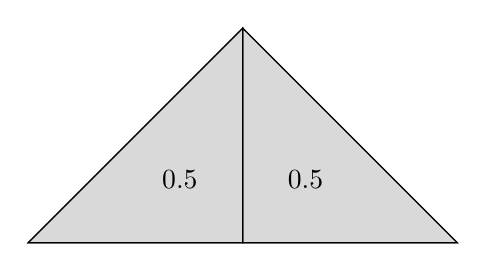
\begin{tikzpicture}[scale=2,baseline={([yshift={-\ht\strutbox}]current bounding box.north)},outer sep=0pt,inner sep=0pt]
            \gemsingem{0.5}{0}
        \end{tikzpicture}
        & The two gems are placed so that their tips touch the container's base and point towards each other. For this table, assume wlog $a_1 \ge a_2$.\\

        \vspace{10pt}

        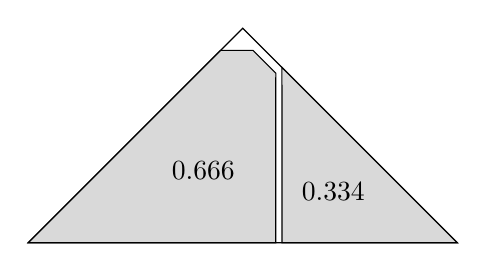
\begin{tikzpicture}[scale=2,baseline={([yshift={-\ht\strutbox}]current bounding box.north)},outer sep=0pt,inner sep=0pt]
            \gemsingem{0.334}{0}
        \end{tikzpicture}
        & They are then pushed as far to the left/to the right as possible.\\

        \vspace{10pt}

        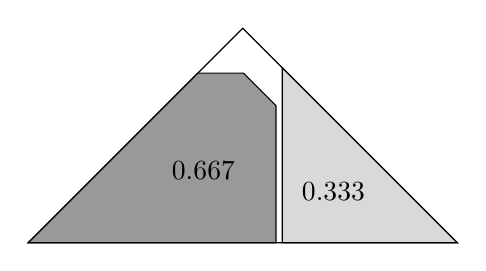
\begin{tikzpicture}[scale=2,baseline={([yshift={-\ht\strutbox}]current bounding box.north)},outer sep=0pt,inner sep=0pt]
            \gemsingem{0.333}{0}
        \end{tikzpicture}
        & As soon as $a_1 > 2 a_2$, we know from REF that $C_1$ will be one single ruby. We no longer need to place a gem container, but we can place the ruby directly.\\

        \vspace{10pt}

        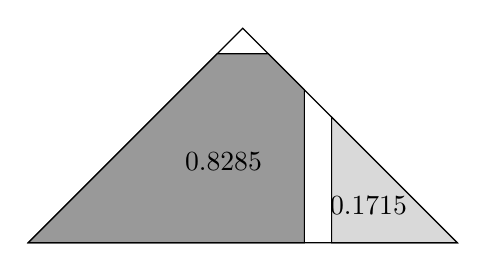
\begin{tikzpicture}[scale=2,baseline={([yshift={-\ht\strutbox}]current bounding box.north)},outer sep=0pt,inner sep=0pt]
            \gemsingem{0.1715}{0}
        \end{tikzpicture}
        & When $a_1 = xxx a_2$, the ruby touches the container's right leg.\\

        \vspace{10pt}

        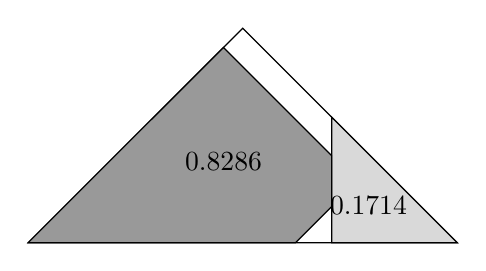
\begin{tikzpicture}[scale=2,baseline={([yshift={-\ht\strutbox}]current bounding box.north)},outer sep=0pt,inner sep=0pt]
            \gemsingem{0.1714}{0}
        \end{tikzpicture}
        & If the ruby gets larger than that, it has to be rotated so that its tip points up.\\

        \vspace{10pt}

        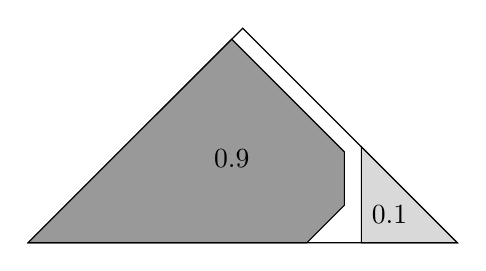
\begin{tikzpicture}[scale=2,baseline={([yshift={-\ht\strutbox}]current bounding box.north)},outer sep=0pt,inner sep=0pt]
            \gemsingem{0.1}{0}
        \end{tikzpicture}
        & \\

        \vspace{10pt}

        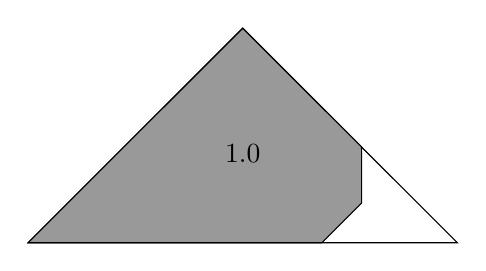
\begin{tikzpicture}[scale=2,baseline={([yshift={-\ht\strutbox}]current bounding box.north)},outer sep=0pt,inner sep=0pt]
            \gemsingem{0}{0}
        \end{tikzpicture}
        & \\
    \end{tabular}
\end{table}

\begin{theorem}
    Any ruby instance $R \in \C(a)$ can be packed into a isosceles right triangle with an incircle of area $a$.
\end{theorem}

\section{Squares}

\begin{lemma}
    The twincircles of a square with area $a$
    have a combined area of
    $\frac{\pi}{3+2\s}a \approx 0.539012a$.
\end{lemma}

\begin{proof}
    We can construct the twincircles' radius $r$ as seen in \Cref{fig:b}:

    \begin{align*}
        2r + 2\frac{r}{\s} &= \sqrt{a}\\
        \iff r &= \frac{\sqrt{a}}{2 + \frac{2}{\s}}\\
    \end{align*}

    So, the combined area of the twincircles is

    $$2\pi r^2 = 2\pi\frac{a}{4 + \frac{8}{\s}+\frac{4}{2}} = \frac{\pi}{3+2\s}a$$
\end{proof}

\begin{figure}[htbp!]
    \centering

    \begin{tikzpicture}[scale=3]
        \squareworstcaseconstruction
    \end{tikzpicture}

    \caption{Construction of the twincircles' radius $r$.}
    \label{fig:b}
\end{figure}

\begin{lemma}
    For any $a'$ larger than a square's twincircle area, there is a circle instance $C \in \C(a')$ that cannot be packed into that square.
\end{lemma}

\begin{proof}
    The instance ${\frac{a'}{2}, \frac{a'}{2}}$ cannot be packed. TODO
\end{proof}

\begin{lemma}\label{th:hatsinsquare}
    Consider a square of area $a$, and set its split key to $F = (1,1)$.
    For all $(F,0)$-rounded tuples $(a_1, b_1)$ and $(a_2, b_2)$ with $a_1 + a_2 \le \frac{\pi}{3+2\s}a$, the following two shapes can be packed into the hat:
    \begin{itemize}
        \item An isosceles right $(a_1,b_1)$-hat and
        \item an isosceles right $(a_2,b_2)$-hat.
    \end{itemize}
\end{lemma}

\begin{figure}[htbp!]
    \centering

    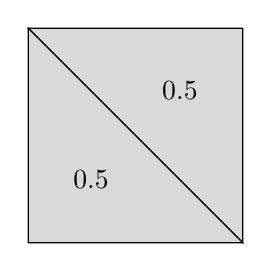
\begin{tikzpicture}[scale=2]
        \hatsinsquare{0.5}
    \end{tikzpicture}
    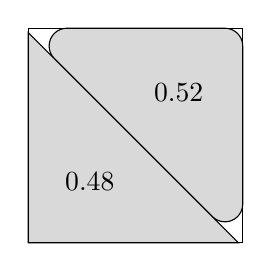
\begin{tikzpicture}[scale=2]
        \hatsinsquare{0.48}
    \end{tikzpicture}
    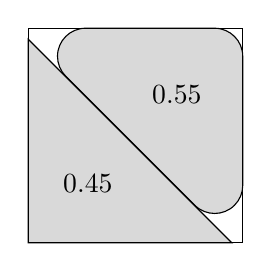
\begin{tikzpicture}[scale=2]
        \hatsinsquare{0.45}
    \end{tikzpicture}
    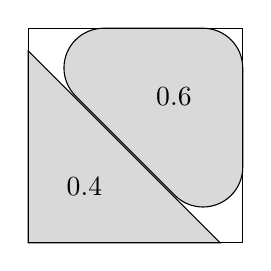
\begin{tikzpicture}[scale=2]
        \hatsinsquare{0.4}
    \end{tikzpicture}

    \vspace{5mm}

    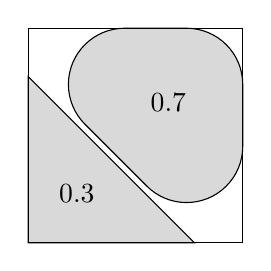
\begin{tikzpicture}[scale=2]
        \hatsinsquare{0.3}
    \end{tikzpicture}
    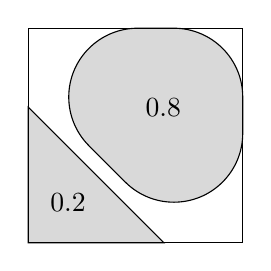
\begin{tikzpicture}[scale=2]
        \hatsinsquare{0.2}
    \end{tikzpicture}
    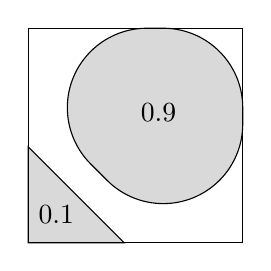
\begin{tikzpicture}[scale=2]
        \hatsinsquare{0.1}
    \end{tikzpicture}
    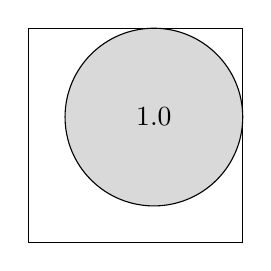
\begin{tikzpicture}[scale=2]
        \hatsinsquare{0}
    \end{tikzpicture}

    \caption{Hat-in-square packings for different values of $a_1$ and $a_2$}
    \label{fig:hatsinsquare}
\end{figure}

\begin{proof}
    Place the tips of the hats in two opposing corners of the square, like in \Cref{fig:hatsinsquare}.
    This placement constitues a valid packing if (1) the hats fit into the square individually and (2) the hats do not overlap.

    We can use the previously established \Cref{th:hatsinhat} for this proof, by only considering the situation above the square's lower-left to upper-right diagonal. If an isosceles right $(\frac{a_1}{2},b_1)$-hat and an isosceless right $(\frac{a_2}{2},b_2)$-hat can be packed into an isosceles right $(\frac{a}{2})$-hat, then this proof is complete.

    As the container hat is symmetric, let $a_1 \ge a_2$.

    $(a_1, b_1)$ and $(a_2, b_2)$ are $(F, 0)$-rounded with $F = (1,1)$. By \Cref{def:rounded}, this means that $b_1 \ge a_1-a_2$. But then also $b_1 \ge \frac{a_1}{2} - \frac{a_2}{2}$, which means that $(\frac{a_1}{2},b_1)$ and $(\frac{a_2}{2},b_2)$ are also $(F, 0)$-rounded, fulfilling the proposition of \Cref{th:hatsinhat}.
\end{proof}

%
%    \begin{itemize}
%        \item[(1)]
%            The hats fit into the square individually if their diagonal never gets larger than the square's edge length $\sqrt{\Psi(x+y)} = \frac{1+\s}{\sqrt{\pi}}\sqrt{x+y}$.
%            As $x \le \frac {x+y} 2$, \Cref{lm:sizes} directly tells us that the $x$-hat has a diagonal of at most
%            \begin{align*}
%                d(x,0) \le d(\frac{x+y}{2},0) = \sqrt{\frac{\frac{x+y}{2}}{\pi}}(2+\s) + 0 = \sqrt{\Psi(x+y)}
%            \end{align*}
%
%            As for the $(y,y-x)$-hat, its diagonal is also never larger than $\sqrt{\Psi(x+y)}$: \todo[inline]{algebraic proof TBD :-)}
%
%            \begin{tikzpicture}
%                \begin{axis}[height=5cm,xtick={0,0.5},xlabel=$\frac{x}{x+y}$,domain=0:0.5,legend pos=outer north east,no markers,samples=500]
%                    \addplot[red,thick] {sqrt((1-x)/pi)*(2+sqrt(2))-sqrt((1-2*x)/pi)*sqrt(2)};
%                    \addplot[blue,thick] {(1+sqrt(2))/sqrt(pi)};
%                    \legend{$\frac{d{(y,y-x)}}{\sqrt{x+y}}$,$\sqrt{\Psi}$}
%                \end{axis} 
%            \end{tikzpicture}
%
%            %\begin{align*}
%            %    d(y,y-x)
%            %    &= \sqrt{\frac{y}{\pi}}(2+\s)-\sqrt{\frac{y-x}{\pi}}\s\\
%            %    &\le \sqrt{\frac{\frac{x+y}{2}}{\pi}}(2+\s)-\sqrt{\frac{y-y}{\pi}}\s\\
%            %    &= \frac{1+\s}{\sqrt{\pi}}\sqrt{x+y} = \sqrt{\Psi(x+y)}
%            %\end{align*}
%
%        \item[(2)]
%            The square has a diagonal of $\sqrt{2a}$.
%            The hats do not overlap if their combined heights never exceeds this diagonal. The height of a right isosceles $a$-hat is $\sqrt{\frac{a}{\pi}}(1+\s)$, and the following inequalities hold:
%
%            \begin{align*}
%                &= \sqrt{\frac{a_1}{\pi}}(1+\s) + \sqrt{\frac{a_2}{\pi}}(1+\s)\\
%                &= \frac{1+\s}{\sqrt\pi}(\sqrt{a_1}+\sqrt{a_2})\\
%                &\le \frac{1+\s}{\sqrt\pi}(\sqrt{2a_1+2a_2})\\
%                &= \s\frac{1+\s}{\sqrt\pi}\sqrt{a_1+a_2}\\
%                &\le \s\frac{1+\s}{\sqrt\pi}\sqrt{\frac{\pi}{3+2\s}a}\\
%                &= \s(1+\s)\sqrt{\frac{1}{(1+\s)^2}a} = \sqrt{2a} \qedhere
%            \end{align*}
%    \end{itemize}
%\end{proof}

%\begin{proof}
%    If $A$ only consists of a single $a$-circle, it can be placed at the center of the square, as its diameter of $2\sqrt{\frac{a}{\pi}} \approx 1.12838\sqrt{a}$ is smaller than the squares edge length $\sqrt{\Psi a} \approx 1.36207\sqrt{a}$. Otherwise, by \Cref{th:split-property}, \textsc{Split} decomposes $A$ into $X \in \C(x)$ and $Y \in \C(y,y-x)$. By \Cref{th:circlesinhat}, we can pack $X$ into a $x$-hat and $Y$ into a $(y,y-x)$-hat. By \Cref{th:hatsinsquare}, we can pack those two hats into the square.
%
%    See \Cref{fig:example} for a complete example packing.
%\end{proof}
%
%\begin{figure}[htbp!]
%    \centering
%    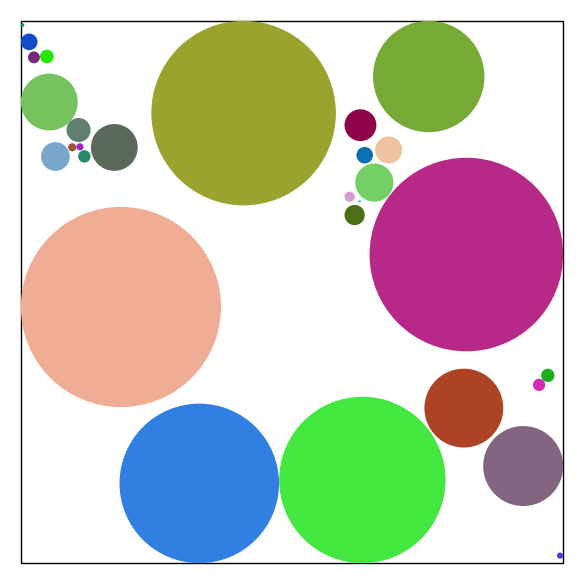
\includegraphics[width=0.5\textwidth]{square_example.png}
%    \caption{Packing of an example instance.}
%    \label{fig:example}
%\end{figure}

\begin{theorem}\label{th:square}
    Any ruby instance with a total area of $a$ can be packed into a square with an area of $xxx a$.
    %A square with an area of $a$ is a $\C(\frac{\pi}{3+2\s}a)$-shape.
\end{theorem}

\begin{proof}
    %By \Cref{th:hatsinsquare} and the Split Packing Theorem.
    If the ruby instance $R$ consists of a single ruby, it can be packed into the square, as its diagonal size is smaller than the square's side length TODO.
    Otherwise, \textsc{Split}$(R, (1,1))$ decomposes $R$ into two subinstances $R_1$ and $R_2$ which can be packed into two $(1,1)$-rounded gems, which, by Lemma TODO can be packed into the square.
\end{proof}

\begin{theorem}
    The Splitpack algorithm, when used to pack circles into squares, is a $\frac{3+2\s}{\pi} \approx 1.85524597$-approximation algorithm, and this factor is tight.
\end{theorem}

\begin{proof}
    When packing a circle instance $C \in \C(a)$ into a square, the smallest possible square container also has area $a$. Indeed, one can construct an instance $C$ which can be packed into a square of area $a+\varepsilon$ by constructing an Apollonian gasket or another asymptotically space-filling circle configuration.

    On the other hand, by \Cref{th:square}, Splitpack packs $C$ into a square of area $\frac{3+2\s}{\pi}a \approx 1.85524597a$.
\end{proof}

\begin{theorem}
    For packing equal circles, Splitpack gives a xxx-approximation.
\end{theorem}

\begin{proof}
    The maximum density for packing equal circles in the plane is $\pi/\sqrt{12}$, so the smallest possible square container has an area of $\frac{\sqrt{12}}{\pi}a$.
\end{proof}

%\chapter{Conclusions and Future Work}

\section{Future Work}

More containers could be considered: Rectangles

The case of acute triangles is still open

Instead of packing circles, other objects could be considered, like ovals or more general convex objects.

Online

Circle-river packing

spheres in cube does not immediately work

\printbibliography

\end{document}
